% *********************************************************************
% © 2016–2019 Jeremy Sylvestre
%
% Permission is granted to copy, distribute and/or modify this document
% under the terms of the GNU Free Documentation License, Version 1.3 or
% any later version published by the Free Software Foundation; with no
% Invariant Sections, no Front-Cover Texts, and no Back-Cover Texts. A
% copy of the license is included in the appendix entitled “GNU Free
% Documentation License” that appears in the output document of this
% PreTeXt source code. All trademarks™ are the registered® marks of
% their respective owners.
%
% *********************************************************************
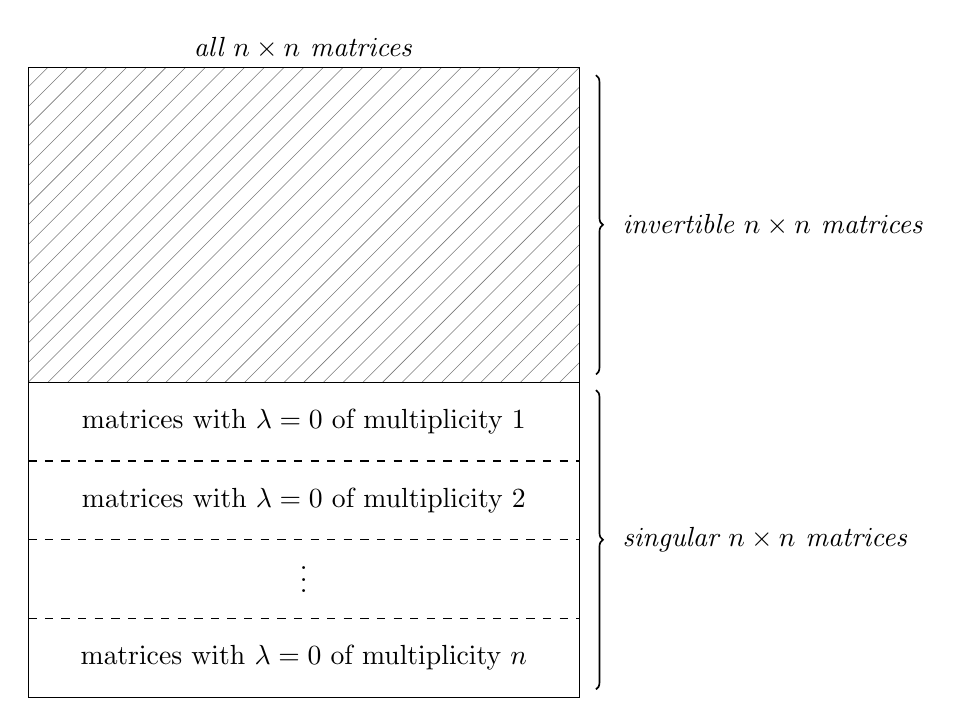
\begin{tikzpicture}

\foreach \x in {0.00,0.25,0.50,...,3.00} {
	\draw[very thin,color=black!5!gray] (\x,4) to (4+\x,8);
}
\foreach \x in {0.25,0.50,0.75,...,3.75} {
	\draw[very thin,color=black!5!gray] (3+\x,4) to (7,8-\x);
}
\foreach \y in {0.25,0.50,0.75,...,3.75} {
	\draw[very thin,color=black!5!gray] (0,4+\y) to (4-\y,8);
}
\draw (0,0) to (7,0) to (7,8) to (0,8) to cycle;
\node at (3.5,8.25) {\textit{all $n \times n$ matrices}};
\draw[dashed] (0,1) to (7,1);
\node at (3.5,0.5) {matrices with $\lambda = 0$ of multiplicity $n$};
\draw[dashed] (0,2) to (7,2);
\node at (3.5,1.6) {$\vdots$};
\draw[dashed] (0,3) to (7,3);
\node at (3.5,2.5) {matrices with $\lambda = 0$ of multiplicity $2$};
\draw (0,4) to (7,4);
\node at (3.5,3.5) {matrices with $\lambda = 0$ of multiplicity $1$};
\draw[semithick,decoration={brace,mirror,raise=6pt},decorate] (7,0.1) -- node[right=12pt] {\textit{singular $n \times n$ matrices}} (7,3.9);
\draw[semithick,decoration={brace,mirror,raise=6pt},decorate] (7,4.1) -- node[right=12pt] {\textit{invertible $n \times n$ matrices}} (7,7.9);

\end{tikzpicture}
